\documentclass[10pt]{article}

\usepackage{fullpage}
\usepackage{setspace}
\usepackage{parskip}
\usepackage{titlesec}
\usepackage{placeins}
\usepackage{xcolor}
\usepackage{breakcites}
\usepackage{lineno}





\PassOptionsToPackage{hyphens}{url}
\usepackage[colorlinks = true,
            linkcolor = blue,
            urlcolor  = blue,
            citecolor = blue,
            anchorcolor = blue]{hyperref}
\usepackage{etoolbox}
\makeatletter
\patchcmd\@combinedblfloats{\box\@outputbox}{\unvbox\@outputbox}{}{%
  \errmessage{\noexpand\@combinedblfloats could not be patched}%
}%
\makeatother


\usepackage[round]{natbib}
\let\cite\citep




\renewenvironment{abstract}
  {{\bfseries\noindent{\abstractname}\par\nobreak}\footnotesize}
  {\bigskip}

\renewenvironment{quote}
  {\begin{tabular}{|p{13cm}}}
  {\end{tabular}}

\titlespacing{\section}{0pt}{*3}{*1}
\titlespacing{\subsection}{0pt}{*2}{*0.5}
\titlespacing{\subsubsection}{0pt}{*1.5}{0pt}


\usepackage{authblk}


\usepackage{graphicx}
\usepackage[space]{grffile}
\usepackage{latexsym}
\usepackage{textcomp}
\usepackage{longtable}
\usepackage{tabulary}
\usepackage{booktabs,array,multirow}
\usepackage{amsfonts,amsmath,amssymb}
\providecommand\citet{\cite}
\providecommand\citep{\cite}
\providecommand\citealt{\cite}
% You can conditionalize code for latexml or normal latex using this.
\newif\iflatexml\latexmlfalse
\providecommand{\tightlist}{\setlength{\itemsep}{0pt}\setlength{\parskip}{0pt}}%

\AtBeginDocument{\DeclareGraphicsExtensions{.pdf,.PDF,.eps,.EPS,.png,.PNG,.tif,.TIF,.jpg,.JPG,.jpeg,.JPEG}}

\usepackage[utf8]{inputenc}
\usepackage[english]{babel}








\begin{document}

\title{PREreview of bioRxiv article ``Convergent evolution of effector protease
recognition by Arabidopsis and barley''}



\author[1]{Sophien Kamoun}%
\affil[1]{The Sainsbury Laboratory}%


\vspace{-1em}



  \date{\today}


\begingroup
\let\center\flushleft
\let\endcenter\endflushleft
\maketitle
\endgroup





\selectlanguage{english}
\begin{abstract}
This is a review of Carter, Helm et al. bioRxiv 374264;
doi:~\url{https://doi.org/10.1101/374264} posted on July 23, 2018. In
this paper, the authors showed that diverse barley cultivars are able to
respond to the Pseudomonas syringae effector AvrPphB and they
characterized~ both the effector target (PBS1) and the receptor (PBR1)
responsible for this recognition. Furthermore, their phylogenetic
analyses revealed that the immune receptor involved in this response is
not orthologous to a previously characterized receptor (RPS5) from
Arabidopsis thaliana that has a functionally analogous AvrPphB
recognition mechanism. This leads the authors to conclude that
recognition of the AvrPphB protease has evolved independently in
Arabidopsis and barley.%
\end{abstract}%




\par\null

\section*{Summary}

{\label{216049}}\par\null

This study builds on previous
publications~\cite{Ade2007}\cite{Zhang2010} that describe the
activity of the Pseudomonas syringae Type 3 host-translocated effector
AvrPphB during infection of Arabidopsis thaliana . AvrPphB is a protease
that cleaves the Arabidopsis receptor like cytoplasmic kinase PBS1,
which in turn is guarded by the nucleotide-binding leucine-rich repeat
(NLR) intracellular receptor RPS5. Upon sensing kinase cleavage by the
effector, RPS5 is activated and triggers the hypersensitive immune
response. Previous studies by Roger Innes group~\cite{Kim2016},
discussed by~\cite{Giannakopoulou2016} have provided a proof of concept for the
use of this system as a platform to develop disease resistance to
diverse plant pathogens. RPS5 recognition spectrum can be broadened by
introducing cleavage sites recognized by different effector proteases
into PBS1. In this paper, the authors explore natural responses to
AvrPphB in plants other than Arabidopsis, notably barley (see Figure
below). They uncovered a recognition system of AvrPphB in barley that is
mechanistically analogous to Arabidopsis RPS5/PBS1 and potentially
exploitable. Two barley orthologs of PBS1, HvPBS1-1 and HvPBS1-2, are
cleaved by AvrPphB. By employing genome-wide association studies (GWAS)
they singled out PBR1, a functional homolog of RPS5, as the NLR that
mediates AvrPphB recognition. They further characterized this PBR1 and
identified a PBR1 homolog in wheat implying that the system could be
functional in this important cereal crop.~

\par\null

We found the paper to be well written and we particularly enjoyed the
original genetic mapping strategies employed to identify the candidate
NLR responsible for AvrPphB recognition. One important implication of
the findings reported by Carter, Helm et al. is that PBS1-derived decoys
can be developed in barley and other cereals such as wheat, to detect
host-translocated protease effectors.\selectlanguage{english}
\begin{figure}[h!]
\begin{center}
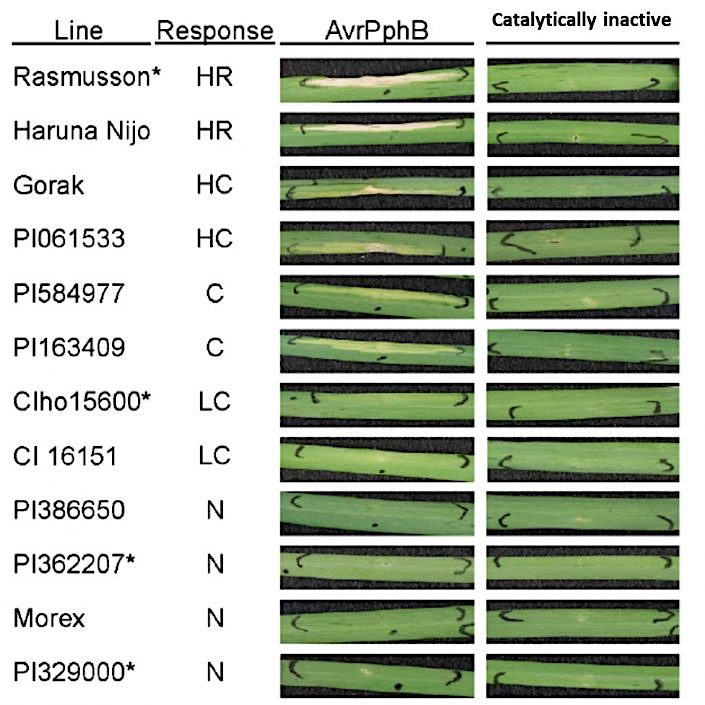
\includegraphics[width=0.70\columnwidth]{figures/AvrPphBcatalytically-inactive-705x705/AvrPphBcatalytically-inactive-705x705}
\caption{{``AvrPphB, and not a catalytically inactive derivative, triggers defense
responses in barley.''~Carter, Helm et al. bioRxiv, 2018.%
}}
\end{center}
\end{figure}

\section*{\(\)Comments}

{\label{457509}}\par\null

\textbf{Phylogenetic analyses.} The authors report that RPS5 and PBR1
are not orthologous based on phylogenetic analysis (Figure 4), and as a
consequence conclude that the capacity to recognize AvrPphB activity is
an example of convergent evolution in Arabidopsis and barley. However,
the phylogenetic trees shown in Fig. 4a and 4b~ lack the broader context
necessary to determine the relatedness of the depicted NLRs.
Phylogenetic analyses that Include a wider diversity of Arabidopsis and
barley NLRs are necessary to conclusively define the evolutionary
relationship between AtRPS5 and PBR1.

\par\null

\textbf{Cell-death assays.} To study PBR1 role in AvrPphB recognition,
the authors carried out cell-death assays (Figure 6) by transiently
expressing both the NLR and the effector in N. benthamiana. However, the
presence of an endogenous PBS1 homolog in these assays limit the level
of mechanistic insight that can be gained from these experiments. We
suggest using a PBS1-silenced or loss-of-function background to obtain
unambiguous results.~

\par\null

\textbf{Figure 2A.} In the experiments depicted in Figure 2A, what was
the rationale behind employing a Bayesian phylogenetic analysis as
opposed to other statistical methods? In general, it would be good to
justify or to mention whether other phylogenetic methods have yielded
similar findings.

\par\null

\textbf{Figure 3A.} In the experiments depicted in Figure 3A, what was
the rationale behind including the barley line with the Low Chlorosis
(LC) response phenotype to AvrPphB in the GWAS as opposed to just using
non-AvrPphB responsive lines?

\(\)

\section*{Reviewers}

{\label{924286}}\par\null

Mauricio P Contreras, Erin K. Zess, and Sophien Kamoun. The Sainsbury
Laboratory, Norwich Research Park, Norwich, UK.

\par\null

\selectlanguage{english}
\FloatBarrier
\bibliographystyle{plainnat}
\bibliography{bibliography/converted_to_latex.bib%
}

\end{document}

